\subsubsection{Các thực thể phục vụ quản lý nguyên liệu}
\label{sec:inventory-data}
Product biểu diễn món bán cho khách; Ingredient biểu diễn tài nguyên thật trong kho. Một nguyên liệu có thể được dùng cho nhiều món, vì vậy không thể coi số phần của mỗi Product là một kho độc lập. Ví dụ cà phê sữa và Americano cùng dùng cà phê rang xay: bán một món sẽ làm giảm khả năng bán món còn lại.

\begin{longtable}{|p{.33\linewidth}|p{.58\linewidth}|}
\hline\textbf{Thành phần} & \textbf{Vai trò và lý do thiết kế}\\\hline\endhead
Ingredient & Lưu id, tên, đơn vị và stock bằng số nguyên theo đơn vị nhỏ nhất (g, ml, cái). Ràng buộc stock không âm bảo vệ dữ liệu ở database.\\\hline
Recipe & Bảng liên kết Product--Ingredient. quantity là định lượng một ly size S; cặp productId/ingredientId duy nhất ngăn khai báo trùng thành phần của cùng công thức. quantity phải dương.\\\hline
Recipe.scalesWithSize & Quyết định lượng có tăng theo size hay không. Cà phê, sữa có thể tăng; ly, nắp thường giữ một cái cho mỗi ly. Không suy ra điều này từ giá bán.\\\hline
ToppingRecipe & Lưu toppingCode, ingredientId và quantity cho một phần topping. Một topping có thể dùng nhiều nguyên liệu; một nguyên liệu có thể vừa thuộc công thức món vừa thuộc topping. Bảng riêng tránh lặp toàn bộ topping cho mỗi món.\\\hline
Order và OrderItem & Order lưu trạng thái và giá trị đơn; OrderItem lưu món, size, topping và số lượng đã chọn. Những lựa chọn này là đầu vào để tính lượng cần giữ.\\\hline
OrderInventoryReservation & Một dòng cho mỗi cặp orderId/ingredientId: quantity lưu chính tổng lượng đã trừ, releasedAt cho biết đã hoàn hay chưa. Đây là snapshot tài nguyên của đơn, không phải công thức sản phẩm thứ hai.\\\hline
Order.reservationExpiresAt & Deadline giữ món được lưu bền vững, dùng chung cho worker, API thanh toán và giao diện. Không phụ thuộc thời điểm khách tải lại trang.\\\hline
Order.reservationExpiredAt & Ghi thời điểm hệ thống đóng do hết hạn; phân biệt với khách chủ động hủy hoặc đơn cũ được thay thế khi đổi món dù đều dùng trạng thái CANCELLED.\\\hline
OrderCreateRequest & Lưu khách, idempotency key, dấu vân tay nội dung và Order kết quả. Ngăn retry tạo thêm đơn và giữ thêm nguyên liệu.\\\hline
\caption{Dữ liệu và trách nhiệm của các bảng trong luồng giữ/hoàn kho}
\end{longtable}

Một Order có nhiều snapshot nguyên liệu; một Ingredient xuất hiện trong snapshot của nhiều Order. Unique(orderId, ingredientId) thể hiện việc cộng gộp trước khi lưu. Quan hệ snapshot tham chiếu nguyên liệu dùng quy tắc Restrict khi xóa, giữ bằng chứng lịch sử ngay cả khi công thức Recipe đã được thay đổi hoặc xóa. OrderItem lưu lựa chọn mua, còn snapshot lưu tài nguyên đã tiêu hao để giữ chỗ: hai loại dữ liệu phục vụ hai mục đích khác nhau.

\begin{sidewaysfigure}\centering
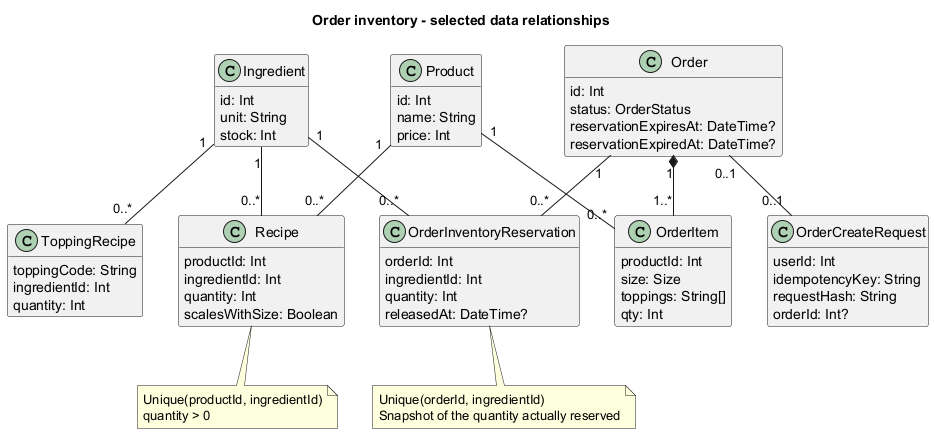
\includegraphics[width=.95\textheight,height=.85\textwidth,keepaspectratio]{assets/inventory/inventory-relations.png}
\caption{Quan hệ dữ liệu của đặt hàng, công thức và snapshot nguyên liệu}
\label{fig:inventory-relations}
\end{sidewaysfigure}
